\documentclass{beamer}

% Theme choice
\usetheme{Madrid}

% Optional packages
\usepackage{graphicx} % For including images
\usepackage{amsmath}  % For math symbols and formulas
\usepackage{hyperref} % For hyperlinks

\title[Deep Learning Tech Introduction]{Deep Learning Tech Introduction}
\author{Nesterov Alexander, Obolenskiy Arseniy}
\institute{ITLab}

\date{\today}

% Redefine the footline to display both the short title and the org name
\setbeamertemplate{footline}{
  \leavevmode%
  \hbox{%
    \begin{beamercolorbox}[wd=.45\paperwidth,ht=2.5ex,dp=1ex,leftskip=1em,center]{author in head/foot}%
        \usebeamerfont{author in head/foot}\insertshortinstitute % Displays the university name
    \end{beamercolorbox}%
    \begin{beamercolorbox}[wd=.45\paperwidth,ht=2.5ex,dp=1ex,leftskip=1em,center]{author in head/foot}%
      \usebeamerfont{author in head/foot}\insertshorttitle % Displays the short title
    \end{beamercolorbox}%
    \begin{beamercolorbox}[wd=.1\paperwidth,ht=2.5ex,dp=1ex,rightskip=1em,center]{author in head/foot}%
      \usebeamerfont{author in head/foot}\insertframenumber{} / \inserttotalframenumber
    \end{beamercolorbox}}%
  \vskip0pt%
}

\begin{document}

\begin{frame}
    \titlepage
\end{frame}

\begin{frame}{Contents}
    \tableofcontents
\end{frame}

\section{Deep neural network}

\begin{frame}{Deep neural network}
  \begin{figure}[h]
    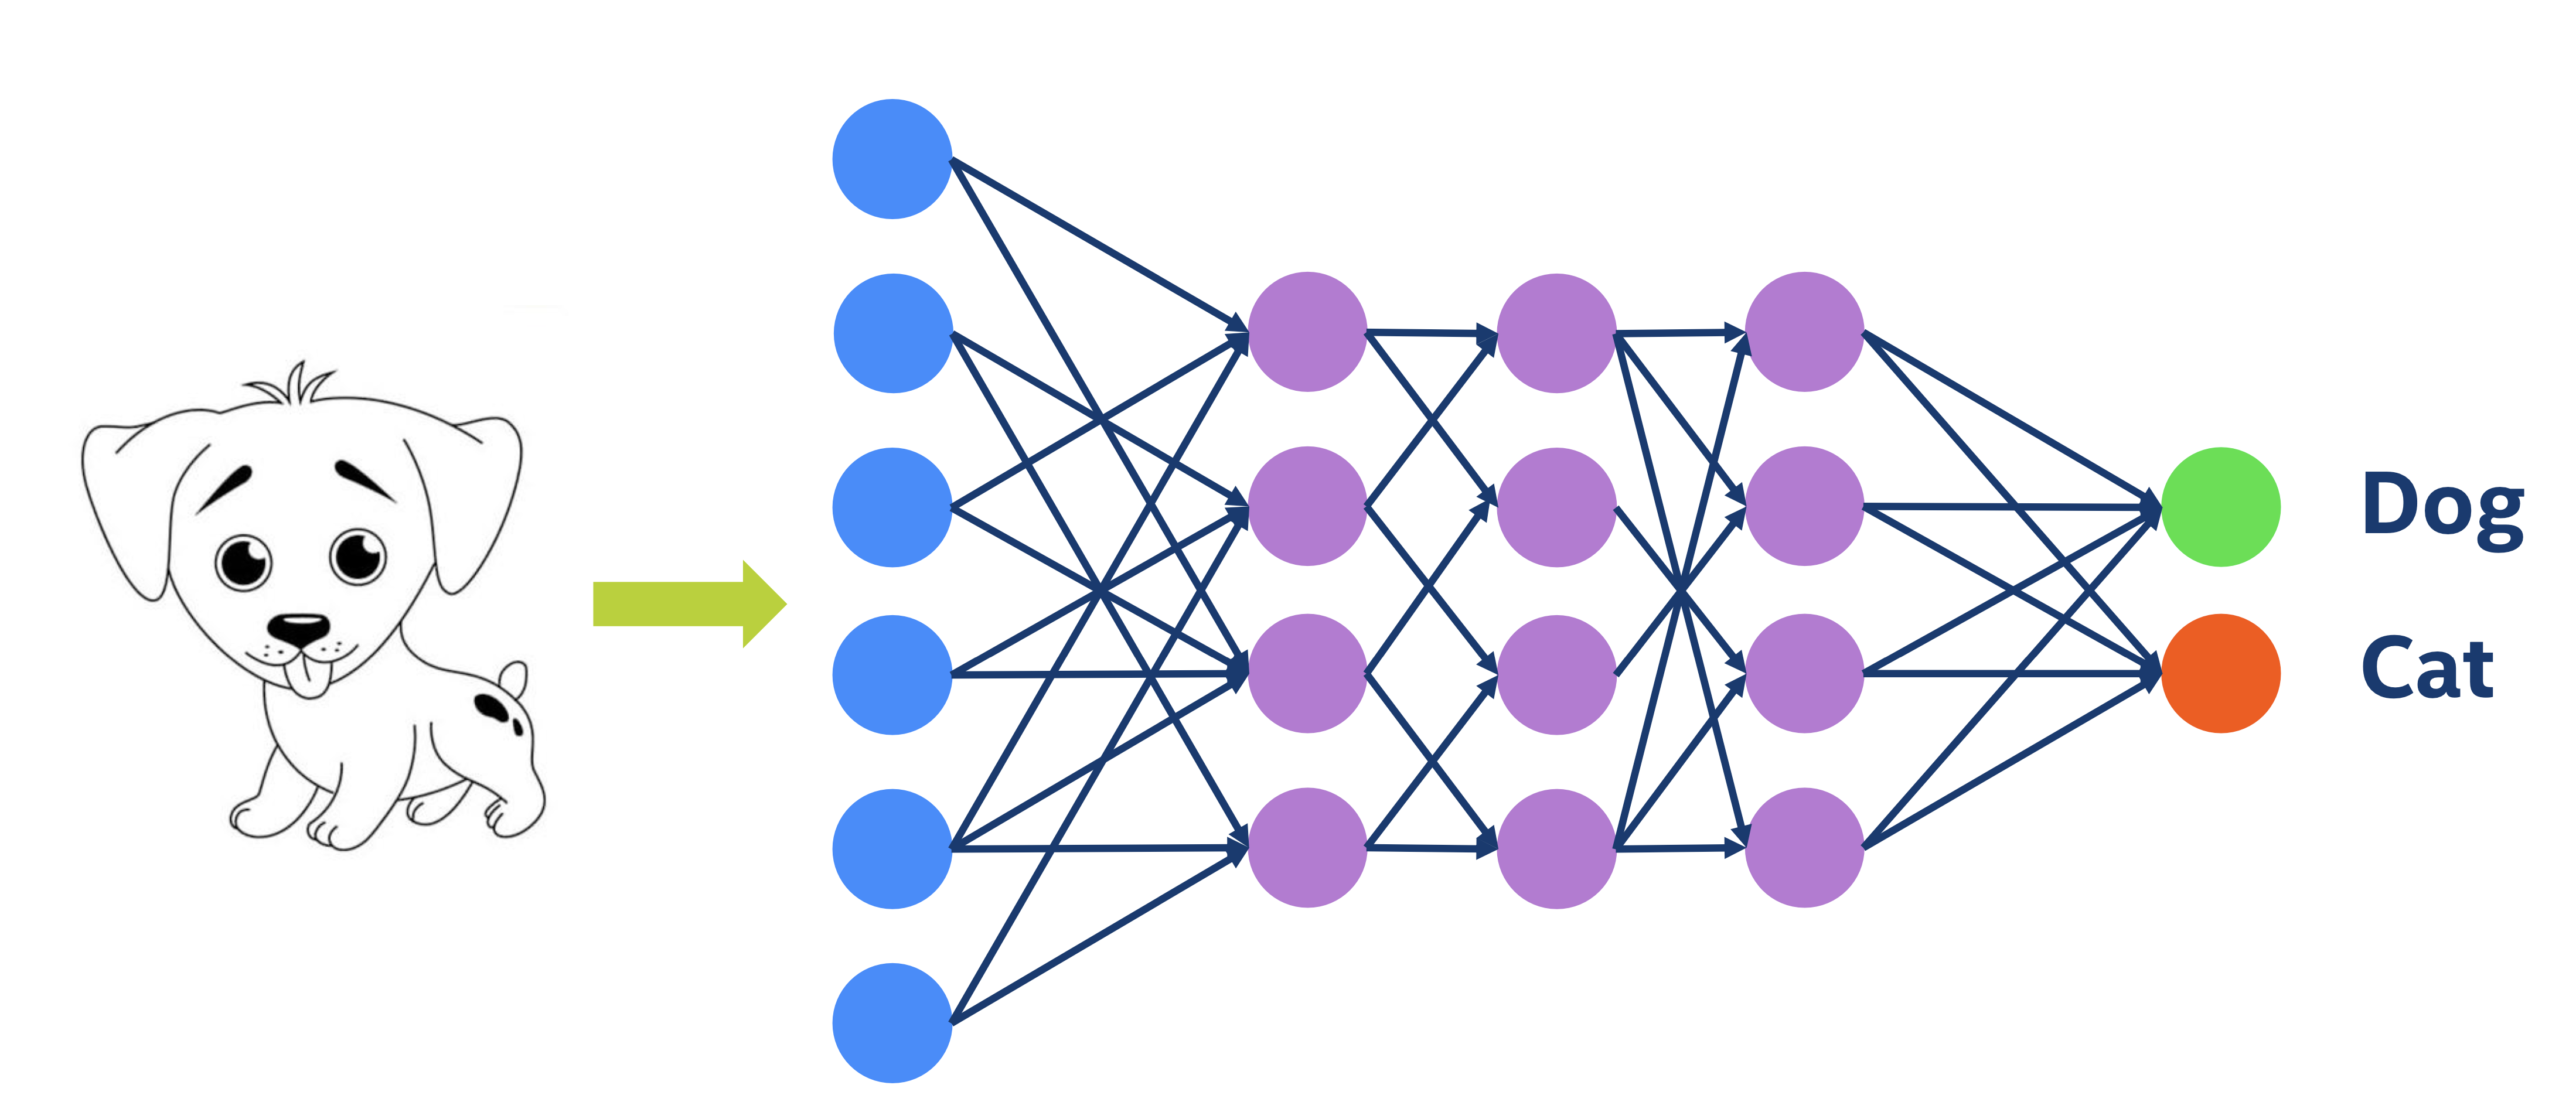
\includegraphics[width=1\textwidth]{images/dnn.png}
  \end{figure}
\end{frame}

\section{What we can to do with DNN?}
\begin{frame}{What we can to do with DNN?}
  \begin{figure}[h]
    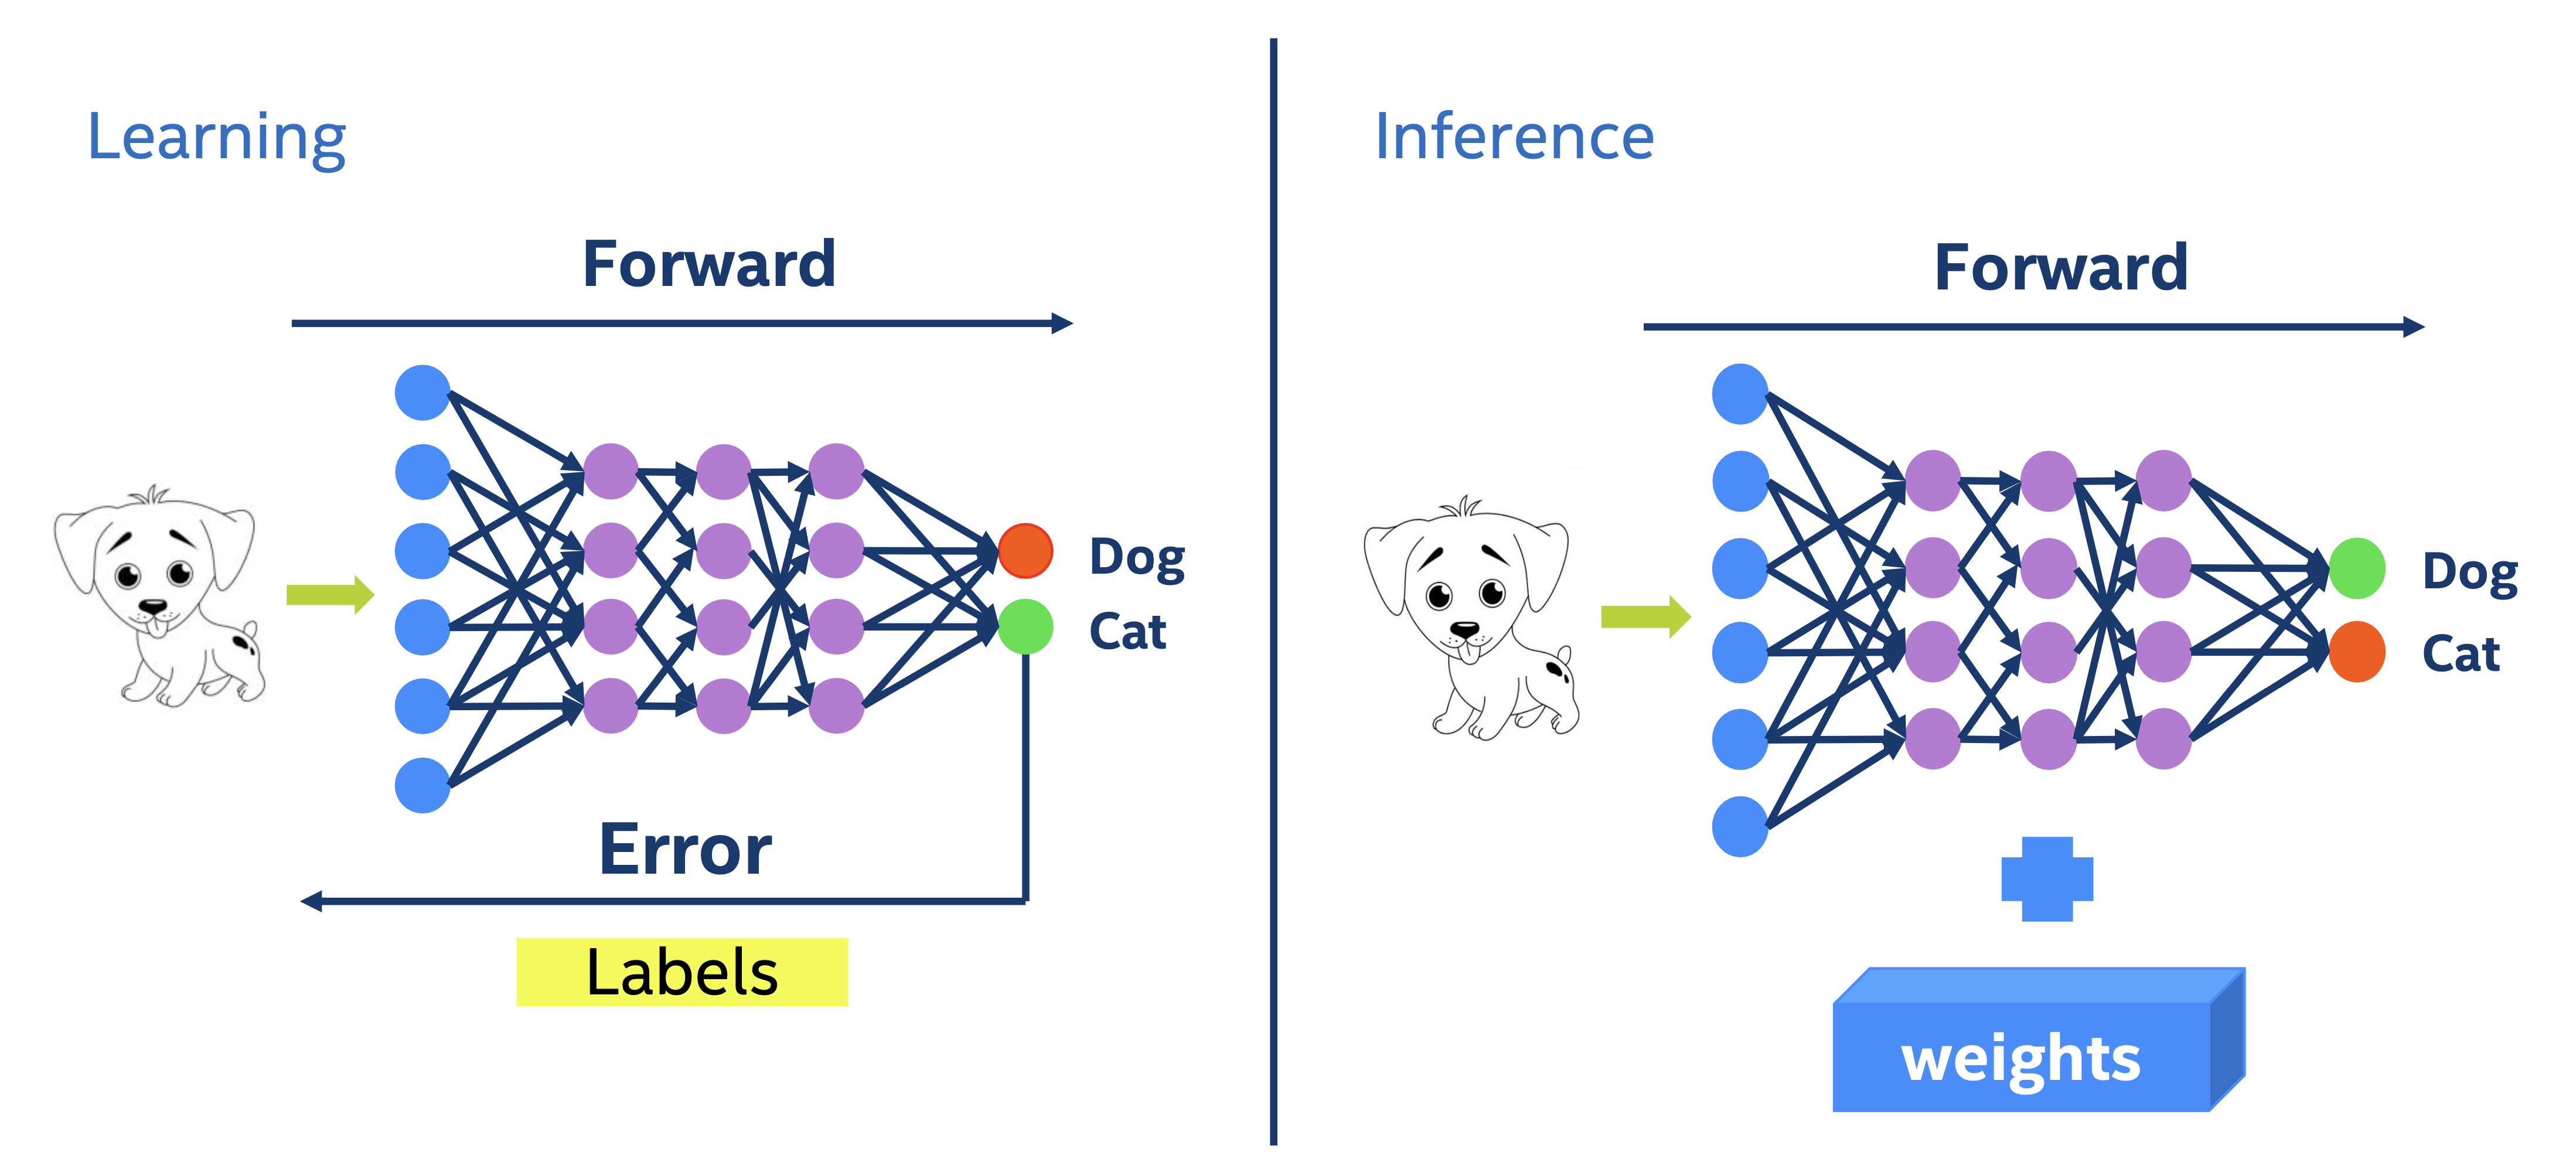
\includegraphics[width=1\textwidth]{images/inference.png}
  \end{figure}
\end{frame}

\section{First network}
\begin{frame}{First network}
  \begin{figure}[h]
    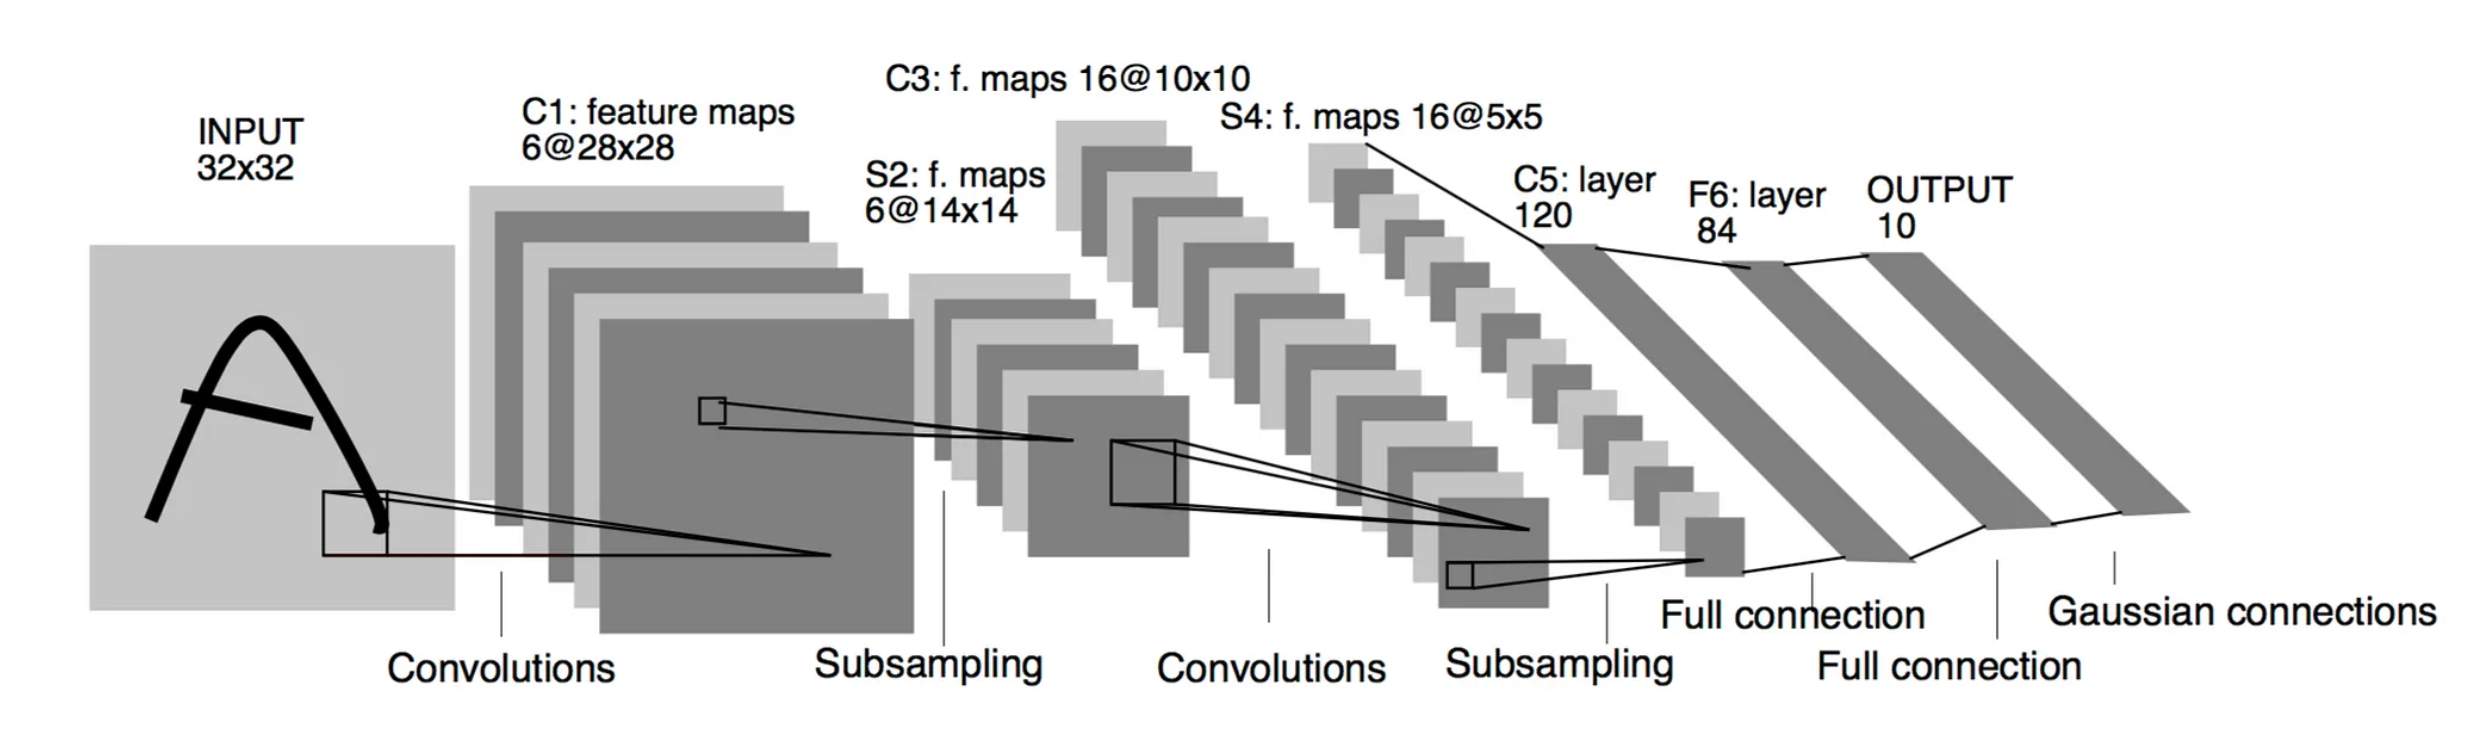
\includegraphics[width=1\textwidth]{images/lenet.png}
  \end{figure}
  \footnotesize Source: \href{https://blog.insightdatascience.com/convolutional-neural-networks-explained-with-american-ninja-warrior-c6649875861c}{Revisiting the LeNet-5 architecture, from “Gradient-Based Learning Applied to Document Recognition” by Yann LeCun et al., Proc. of the IEEE, 1998.}
\end{frame}

\section{Frameworks}
\begin{frame}{Frameworks}
  \begin{figure}[h]
    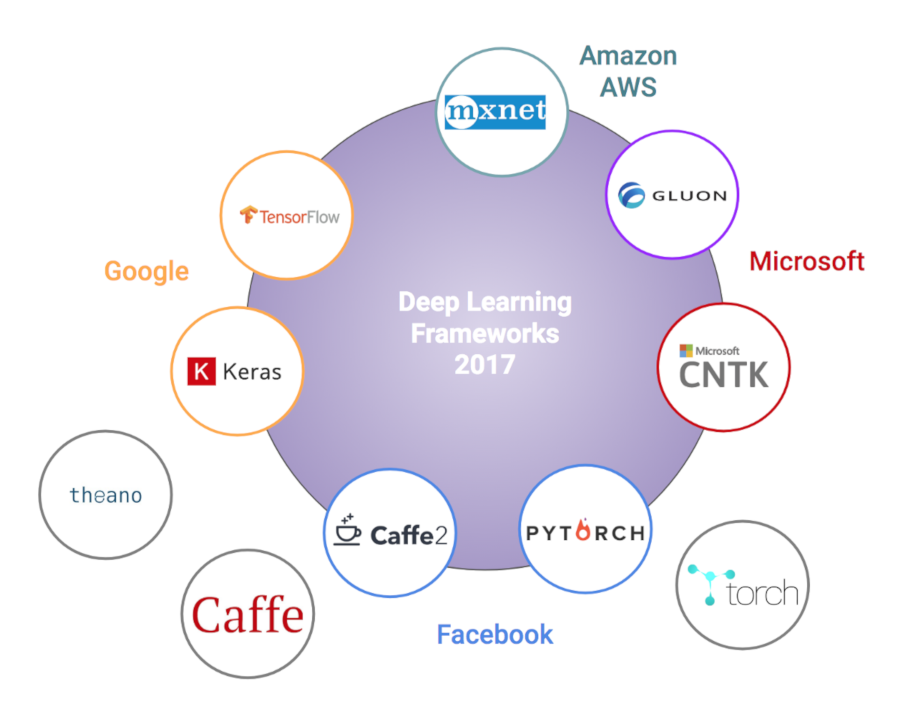
\includegraphics[width=0.85\textwidth]{images/frameworks.png}
  \end{figure}
  \footnotesize Source: \href{https://devopedia.org/deep-learning-frameworks}{Battle of the Deep Learning frameworks Part 1: 2017, even more frameworks and interfaces. Towards Data Science, December 19. Accessed 2019-01-20.}
\end{frame}

\section{OpenVINO - Small IR}
\begin{frame}{OpenVINO - Small IR}
  \begin{figure}[h]
    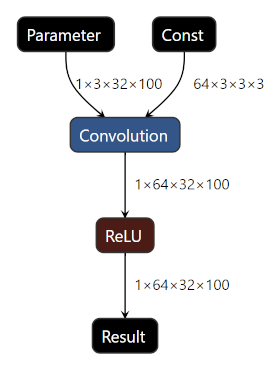
\includegraphics[width=0.4\textwidth]{images/small_ir.png}
  \end{figure}
  \footnotesize Source: \href{https://docs.openvino.ai/}{docs.openvino.ai}
\end{frame}

\section{OpenVINO - Netron}
\begin{frame}{OpenVINO - Netron}
  \begin{figure}[h]
    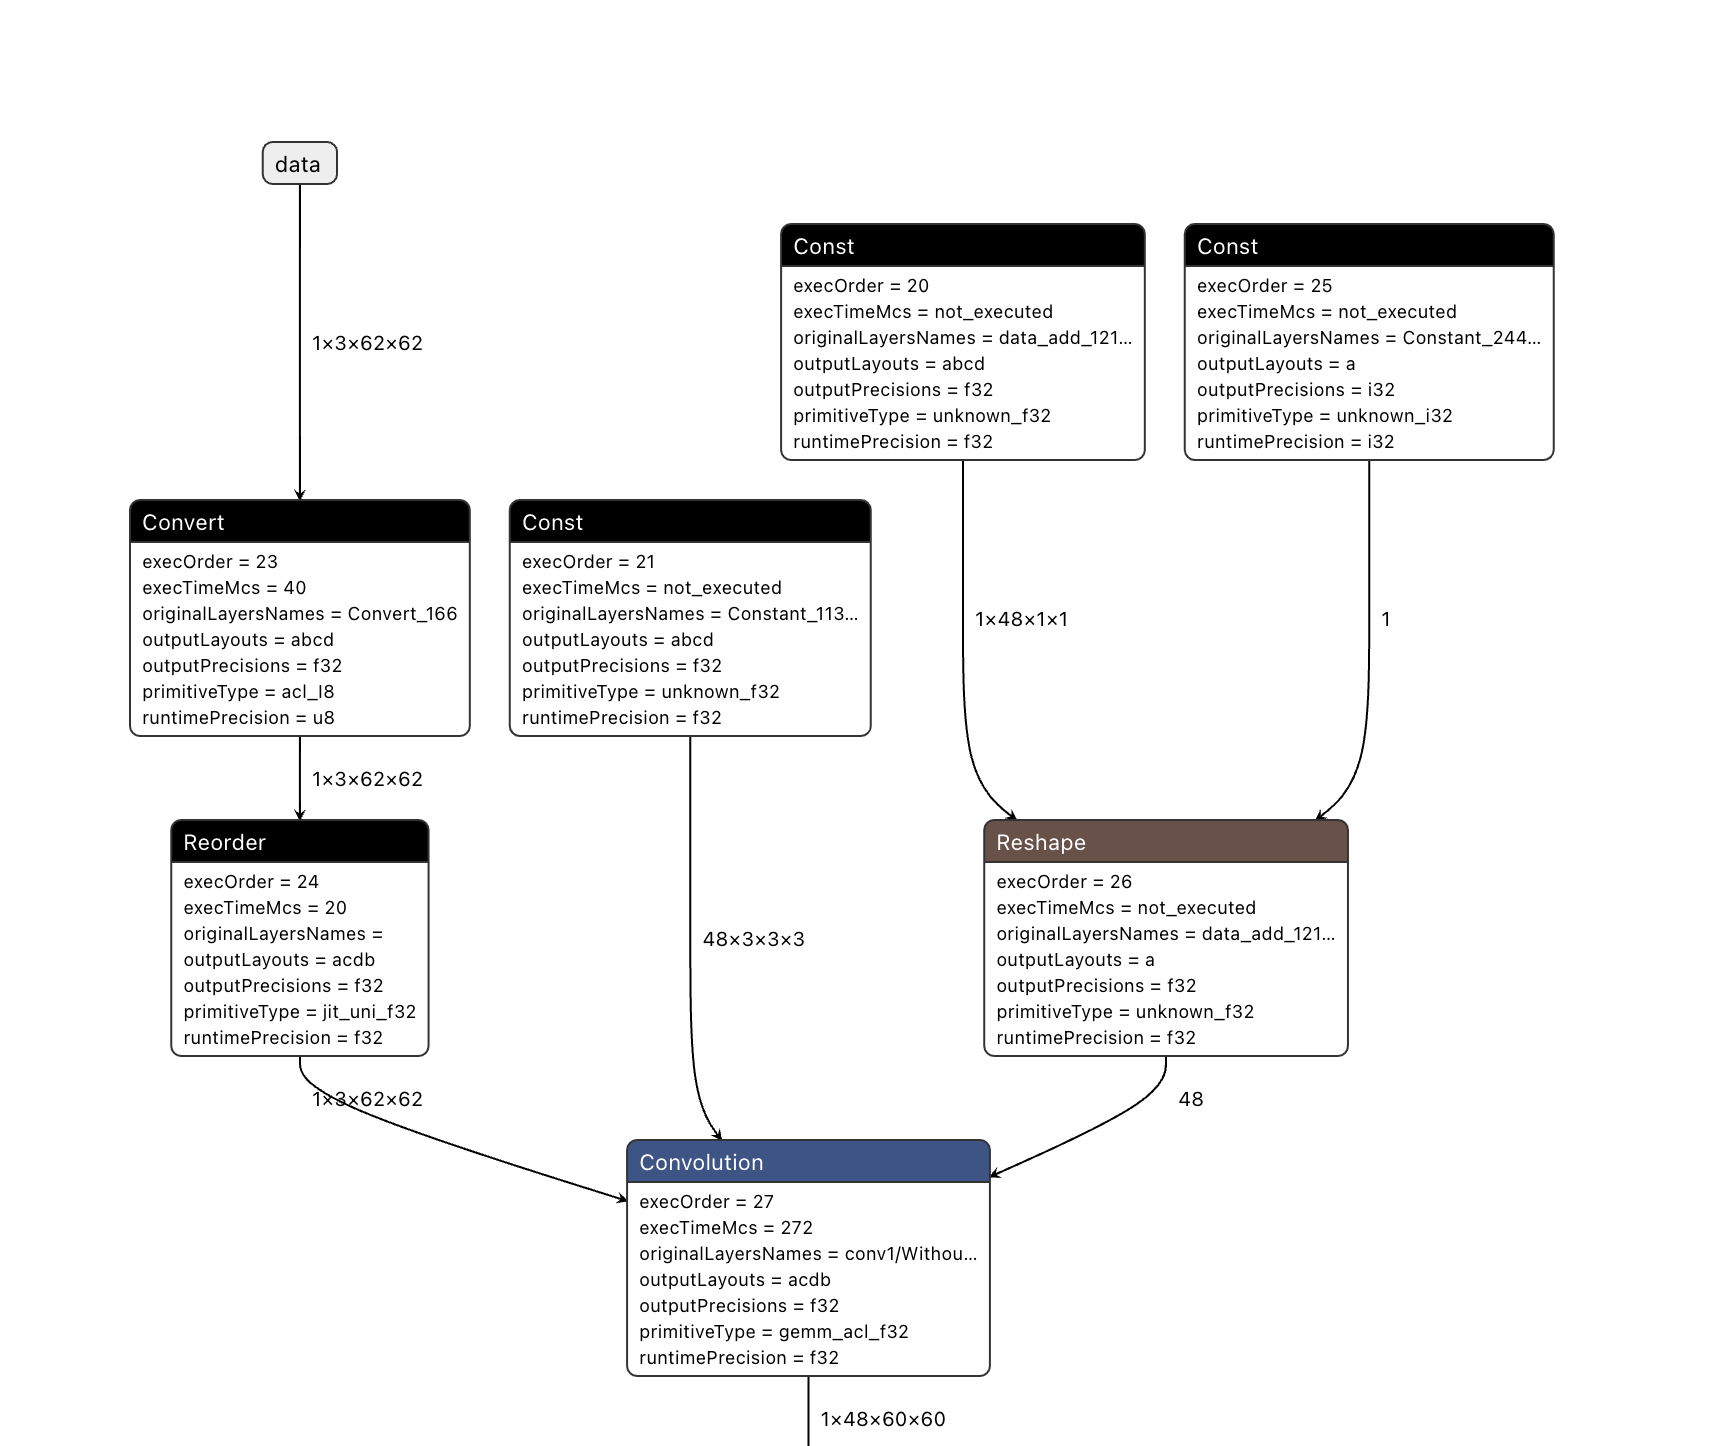
\includegraphics[width=0.6\textwidth]{images/openvino.png}
  \end{figure}
  \footnotesize Source: \href{https://netron.app/}{netron.app}
\end{frame}

\section{What next?}
\begin{frame}{What next?}
  \begin{itemize}
    \item Arm Compute Library (ACL) - what is it?
    \item Layers representation in ACL
    \item First Examples
  \end{itemize}
\end{frame}

\end{document}
